% Options for packages loaded elsewhere
\PassOptionsToPackage{unicode}{hyperref}
\PassOptionsToPackage{hyphens}{url}
%
\documentclass[
  letterpaper,
  oneside,
  open=any]{scrbook}

\usepackage{amsmath,amssymb}
\usepackage{iftex}
\ifPDFTeX
  \usepackage[T1]{fontenc}
  \usepackage[utf8]{inputenc}
  \usepackage{textcomp} % provide euro and other symbols
\else % if luatex or xetex
  \usepackage{unicode-math}
  \defaultfontfeatures{Scale=MatchLowercase}
  \defaultfontfeatures[\rmfamily]{Ligatures=TeX,Scale=1}
\fi
\usepackage{lmodern}
\ifPDFTeX\else  
    % xetex/luatex font selection
\fi
% Use upquote if available, for straight quotes in verbatim environments
\IfFileExists{upquote.sty}{\usepackage{upquote}}{}
\IfFileExists{microtype.sty}{% use microtype if available
  \usepackage[]{microtype}
  \UseMicrotypeSet[protrusion]{basicmath} % disable protrusion for tt fonts
}{}
\makeatletter
\@ifundefined{KOMAClassName}{% if non-KOMA class
  \IfFileExists{parskip.sty}{%
    \usepackage{parskip}
  }{% else
    \setlength{\parindent}{0pt}
    \setlength{\parskip}{6pt plus 2pt minus 1pt}}
}{% if KOMA class
  \KOMAoptions{parskip=half}}
\makeatother
\usepackage{xcolor}
\setlength{\emergencystretch}{3em} % prevent overfull lines
\setcounter{secnumdepth}{5}
% Make \paragraph and \subparagraph free-standing
\ifx\paragraph\undefined\else
  \let\oldparagraph\paragraph
  \renewcommand{\paragraph}[1]{\oldparagraph{#1}\mbox{}}
\fi
\ifx\subparagraph\undefined\else
  \let\oldsubparagraph\subparagraph
  \renewcommand{\subparagraph}[1]{\oldsubparagraph{#1}\mbox{}}
\fi

\providecommand{\tightlist}{%
  \setlength{\itemsep}{0pt}\setlength{\parskip}{0pt}}\usepackage{longtable,booktabs,array}
\usepackage{calc} % for calculating minipage widths
% Correct order of tables after \paragraph or \subparagraph
\usepackage{etoolbox}
\makeatletter
\patchcmd\longtable{\par}{\if@noskipsec\mbox{}\fi\par}{}{}
\makeatother
% Allow footnotes in longtable head/foot
\IfFileExists{footnotehyper.sty}{\usepackage{footnotehyper}}{\usepackage{footnote}}
\makesavenoteenv{longtable}
\usepackage{graphicx}
\makeatletter
\def\maxwidth{\ifdim\Gin@nat@width>\linewidth\linewidth\else\Gin@nat@width\fi}
\def\maxheight{\ifdim\Gin@nat@height>\textheight\textheight\else\Gin@nat@height\fi}
\makeatother
% Scale images if necessary, so that they will not overflow the page
% margins by default, and it is still possible to overwrite the defaults
% using explicit options in \includegraphics[width, height, ...]{}
\setkeys{Gin}{width=\maxwidth,height=\maxheight,keepaspectratio}
% Set default figure placement to htbp
\makeatletter
\def\fps@figure{htbp}
\makeatother
% definitions for citeproc citations
\NewDocumentCommand\citeproctext{}{}
\NewDocumentCommand\citeproc{mm}{%
  \begingroup\def\citeproctext{#2}\cite{#1}\endgroup}
\makeatletter
 % allow citations to break across lines
 \let\@cite@ofmt\@firstofone
 % avoid brackets around text for \cite:
 \def\@biblabel#1{}
 \def\@cite#1#2{{#1\if@tempswa , #2\fi}}
\makeatother
\newlength{\cslhangindent}
\setlength{\cslhangindent}{1.5em}
\newlength{\csllabelwidth}
\setlength{\csllabelwidth}{3em}
\newenvironment{CSLReferences}[2] % #1 hanging-indent, #2 entry-spacing
 {\begin{list}{}{%
  \setlength{\itemindent}{0pt}
  \setlength{\leftmargin}{0pt}
  \setlength{\parsep}{0pt}
  % turn on hanging indent if param 1 is 1
  \ifodd #1
   \setlength{\leftmargin}{\cslhangindent}
   \setlength{\itemindent}{-1\cslhangindent}
  \fi
  % set entry spacing
  \setlength{\itemsep}{#2\baselineskip}}}
 {\end{list}}
\usepackage{calc}
\newcommand{\CSLBlock}[1]{\hfill\break\parbox[t]{\linewidth}{\strut\ignorespaces#1\strut}}
\newcommand{\CSLLeftMargin}[1]{\parbox[t]{\csllabelwidth}{\strut#1\strut}}
\newcommand{\CSLRightInline}[1]{\parbox[t]{\linewidth - \csllabelwidth}{\strut#1\strut}}
\newcommand{\CSLIndent}[1]{\hspace{\cslhangindent}#1}

\usepackage[default]{opensans}
\fontseries{lc}\selectfont
\makeatletter
\@ifpackageloaded{bookmark}{}{\usepackage{bookmark}}
\makeatother
\makeatletter
\@ifpackageloaded{caption}{}{\usepackage{caption}}
\AtBeginDocument{%
\ifdefined\contentsname
  \renewcommand*\contentsname{Table of contents}
\else
  \newcommand\contentsname{Table of contents}
\fi
\ifdefined\listfigurename
  \renewcommand*\listfigurename{List of Figures}
\else
  \newcommand\listfigurename{List of Figures}
\fi
\ifdefined\listtablename
  \renewcommand*\listtablename{List of Tables}
\else
  \newcommand\listtablename{List of Tables}
\fi
\ifdefined\figurename
  \renewcommand*\figurename{Figure}
\else
  \newcommand\figurename{Figure}
\fi
\ifdefined\tablename
  \renewcommand*\tablename{Table}
\else
  \newcommand\tablename{Table}
\fi
}
\@ifpackageloaded{float}{}{\usepackage{float}}
\floatstyle{ruled}
\@ifundefined{c@chapter}{\newfloat{codelisting}{h}{lop}}{\newfloat{codelisting}{h}{lop}[chapter]}
\floatname{codelisting}{Listing}
\newcommand*\listoflistings{\listof{codelisting}{List of Listings}}
\makeatother
\makeatletter
\makeatother
\makeatletter
\@ifpackageloaded{caption}{}{\usepackage{caption}}
\@ifpackageloaded{subcaption}{}{\usepackage{subcaption}}
\makeatother

\usepackage{hyphenat}
\usepackage{ifthen}
\usepackage{calc}
\usepackage{calculator}

\usepackage{graphicx}
\usepackage{wallpaper}

\usepackage{geometry}

\usepackage{graphicx}
\usepackage{geometry}
\usepackage{afterpage}
\usepackage{tikz}
\usetikzlibrary{calc}
\usetikzlibrary{fadings}
\usepackage[pagecolor=none]{pagecolor}


% Set the titlepage font families







% Set the coverpage font families

\ifLuaTeX
  \usepackage{selnolig}  % disable illegal ligatures
\fi
\usepackage{bookmark}

\IfFileExists{xurl.sty}{\usepackage{xurl}}{} % add URL line breaks if available
\urlstyle{same} % disable monospaced font for URLs
\hypersetup{
  pdftitle={CPS Acoustic Classification},
  pdfauthor={Alice Beittel},
  hidelinks,
  pdfcreator={LaTeX via pandoc}}

\title{CPS Acoustic Classification}
\author{Alice Beittel}
\date{}

\begin{document}
%%%%% begin titlepage extension code

  \begin{frontmatter}

\begin{titlepage}
% This is a combination of Pandoc templating and LaTeX
% Pandoc templating https://pandoc.org/MANUAL.html#templates
% See the README for help

\thispagestyle{empty}

\newgeometry{top=-100in}

% Page color

\newcommand{\coverauthorstyle}[1]{{\fontsize{20}{24.0}\selectfont
#1}}

\begin{tikzpicture}[remember picture, overlay, inner sep=0pt, outer sep=0pt]

\tikzfading[name=fadeout, inner color=transparent!0,outer color=transparent!100]
\tikzfading[name=fadein, inner color=transparent!100,outer color=transparent!0]
\node[anchor=south west, rotate=0.0, opacity=1.0] at ($(current page.south west)+(0pt, 8.75in)$) {

\includegraphics[width=\paperwidth, keepaspectratio]{images/cover-header-2.png}};

% Title
\newcommand{\titlelocationleft}{2.3in}
\newcommand{\titlelocationbottom}{7in}
\newcommand{\titlealign}{left}

\begin{scope}{%
\fontsize{30}{36.0}\selectfont
\node[anchor=north
west, align=left, rotate=0] (Title1) at ($(current page.south west)+(\titlelocationleft,\titlelocationbottom)$)  [text width = 5in]  {\textcolor{black}{\bfseries{\nohyphens{CPS
Acoustic Classification}}}};
}
\end{scope}

% Author
\newcommand{\authorlocationleft}{2.3in}
\newcommand{\authorlocationbottom}{5in}
\newcommand{\authoralign}{left}

\begin{scope}
{%
\fontsize{20}{24.0}\selectfont
\node[anchor=north
west, align=left, rotate=0] (Author1) at ($(current page.south west)+(\authorlocationleft,\authorlocationbottom)$)  [text width = 5in]  {
\coverauthorstyle{Alice Beittel\\}};
}
\end{scope}

% Header
\newcommand{\headerlocationleft}{2.3in}
\newcommand{\headerlocationbottom}{9.8in}
\newcommand{\headerlocationalign}{left}

\begin{scope}
{%
\fontsize{16}{19.2}\selectfont
 \node[anchor=north west, align=left, rotate=0] (Header1) at %
($(current page.south west)+(\headerlocationleft,\headerlocationbottom)$)  [text width = 5in]  {\textcolor{white}{\nohyphens{NOAA
Technical Memorandum NMFS-XXX-\#\#}}};
}
\end{scope}

% Footer
\newcommand{\footerlocationleft}{6in}
\newcommand{\footerlocationbottom}{0.1\paperheight}
\newcommand{\footerlocationalign}{left}

\begin{scope}
{%
\fontsize{8}{9.6}\selectfont
 \node[anchor=north west, align=left, rotate=0] (Footer1) at %
($(current page.south west)+(\footerlocationleft,\footerlocationbottom)$)  [text width = 2.5in]  {{\nohyphens{U.S.
DEPARTMENT OF COMMERCE\\
\strut \\
National Oceanic and Atmospheric Administration\\
National Marine Fisheries Service\\
Northwest Fisheries Science Center}}};
}
\end{scope}

% Date
\newcommand{\datelocationleft}{6in}
\newcommand{\datelocationbottom}{2in}
\newcommand{\datelocationalign}{left}

\begin{scope}
{%
\fontsize{20}{24.0}\selectfont
 \node[anchor=north west, align=left, rotate=0] (Date1) at %
($(current page.south west)+(\datelocationleft,\datelocationbottom)$)  [text width = 2.5in]  {{\nohyphens{January
2023}}};
}
\end{scope}

\end{tikzpicture}
\clearpage
\restoregeometry
%%% TITLE PAGE START

% Set up alignment commands
%Page
\newcommand{\titlepagepagealign}{
\ifthenelse{\equal{left}{right}}{\raggedleft}{}
\ifthenelse{\equal{left}{center}}{\centering}{}
\ifthenelse{\equal{left}{left}}{\raggedright}{}
}
%% Titles
\newcommand{\titlepagetitlealign}{
\ifthenelse{\equal{left}{right}}{\raggedleft}{}
\ifthenelse{\equal{left}{center}}{\centering}{}
\ifthenelse{\equal{left}{left}}{\raggedright}{}
\ifthenelse{\equal{left}{spread}}{\makebox[\linewidth][s]}{}
}


\newcommand{\titleandsubtitle}{
% Title and subtitle
{\fontsize{30}{36.0}\selectfont
\textcolor{black}{\bfseries{\nohyphens{CPS Acoustic
Classification}}}\par
}%
}
\newcommand{\titlepagetitleblock}{
\titleandsubtitle
}

\newcommand{\authorstyle}[1]{{\fontsize{20}{24.0}\selectfont
#1}}

\newcommand{\affiliationstyle}[1]{{#1}}

\newcommand{\titlepageauthorblock}{
{\authorstyle{\nohyphens{Alice Beittel}{\textsuperscript{1}}}}}

\newcommand{\titlepageaffiliationblock}{
\hangindent=1em
\hangafter=1
{\affiliationstyle{
{1}.~NOAA Southwest Fisheres Science Center,~Southwest Fisheries Science
Center


\vspace{1\baselineskip} 
}}
}
\newcommand{\headerstyled}{%
{}
}
\newcommand{\footerstyled}{%
{}
}
\newcommand{\datestyled}{%
{}
}


\newcommand{\titlepageheaderblock}{\headerstyled}

\newcommand{\titlepagefooterblock}{
\footerstyled
}

\newcommand{\titlepagedateblock}{
\datestyled
}

%set up blocks so user can specify order
\newcommand{\titleblock}{{\titlepagetitlealign

{\titlepagetitleblock}
}

\vspace{4\baselineskip}
}

\newcommand{\authorblock}{{\titlepageauthorblock}

\vspace{2\baselineskip}
}

\newcommand{\affiliationblock}{{\titlepageaffiliationblock}

\vspace{2\baselineskip}
}

\newcommand{\logoblock}{}

\newcommand{\footerblock}{}

\newcommand{\dateblock}{}

\newcommand{\headerblock}{}
\newgeometry{top=3in,bottom=1in,right=1in,left=1.75in}
% background image
\newlength{\bgimagesize}
\setlength{\bgimagesize}{0.75\paperwidth}
\LENGTHDIVIDE{\bgimagesize}{\paperwidth}{\theRatio} % from calculator pkg
\ThisULCornerWallPaper{\theRatio}{images/corner-image.png}

\thispagestyle{empty} % no page numbers on titlepages


\newcommand{\vrulecode}{\rule{\vrulewidth}{\textheight}}
\newlength{\vrulewidth}
\setlength{\vrulewidth}{0pt}
\newlength{\B}
\setlength{\B}{\ifdim\vrulewidth > 0pt 0.05\textwidth\else 0pt\fi}
\newlength{\minipagewidth}
\ifthenelse{\equal{left}{left} \OR \equal{left}{right} }
{% True case
\setlength{\minipagewidth}{\textwidth - \vrulewidth - \B - 0.1\textwidth}
}{
\setlength{\minipagewidth}{\textwidth - 2\vrulewidth - 2\B - 0.1\textwidth}
}
\ifthenelse{\equal{left}{left} \OR \equal{left}{leftright}}
{% True case
\raggedleft % needed for the minipage to work
\vrulecode
\hspace{\B}
}{%
\raggedright % else it is right only and width is not 0
}
% [position of box][box height][inner position]{width}
% [s] means stretch out vertically; assuming there is a vfill
\begin{minipage}[b][\textheight][s]{\minipagewidth}
\titlepagepagealign
\headerblock

\titleblock

\authorblock

\affiliationblock

\vfill

\logoblock

\footerblock
\par

\end{minipage}\ifthenelse{\equal{left}{right} \OR \equal{left}{leftright} }{
\hspace{\B}
\vrulecode}{}
\clearpage
\restoregeometry
%%% TITLE PAGE END
\end{titlepage}
\setcounter{page}{1}
\end{frontmatter}

%%%%% end titlepage extension code

\renewcommand*\contentsname{Table of contents}
{
\setcounter{tocdepth}{1}
\tableofcontents
}
\listoffigures
\listoftables
\mainmatter
\bookmarksetup{startatroot}

\chapter*{Welcome}\label{welcome}
\addcontentsline{toc}{chapter}{Welcome}

\markboth{Welcome}{Welcome}

\textbf{Last updated:} 2024-12-18 10:46:18 PST

\href{https://www.fisheries.noaa.gov/species/west-coast-coastal-pelagic-species}{West
Coast coastal pelagic species} play an important role in the California
Current ecosystem. They're food sources for marine mammals, sea birds,
and larger fish, and they support commercial and recreational fisheries
(J. Zwolinski et al. 2014). Each year the NOAA Southwest Fisheries
Science Center surveys the west coast from Baja Mexico to Vancouver
Island, Canada to measure the biomass of 5 key coastal pelagic species:
\href{https://www.fisheries.noaa.gov/species/pacific-sardine\#:~:text=Baja\%20California\%2C\%20Mexico.-,Habitat,schools\%20near\%20the\%20ocean\%20surface.}{Pacific
Sardine} \emph{Sardinops sagax}, Northern Anchovy \emph{Engraulis
mordax}, Pacific Mackerel \emph{Scomber japonicus,} Jack Mackerel
\emph{Trachurus symmetricus,} Pacific Herring \emph{Clupea pallasii,}
and Round Herring \emph{Etrumeus acuminatus}. The biomass and abundance
estimates derived from the survey are used in stock assessment models to
support sustainable fisheries.

\begin{figure}[H]

{\centering 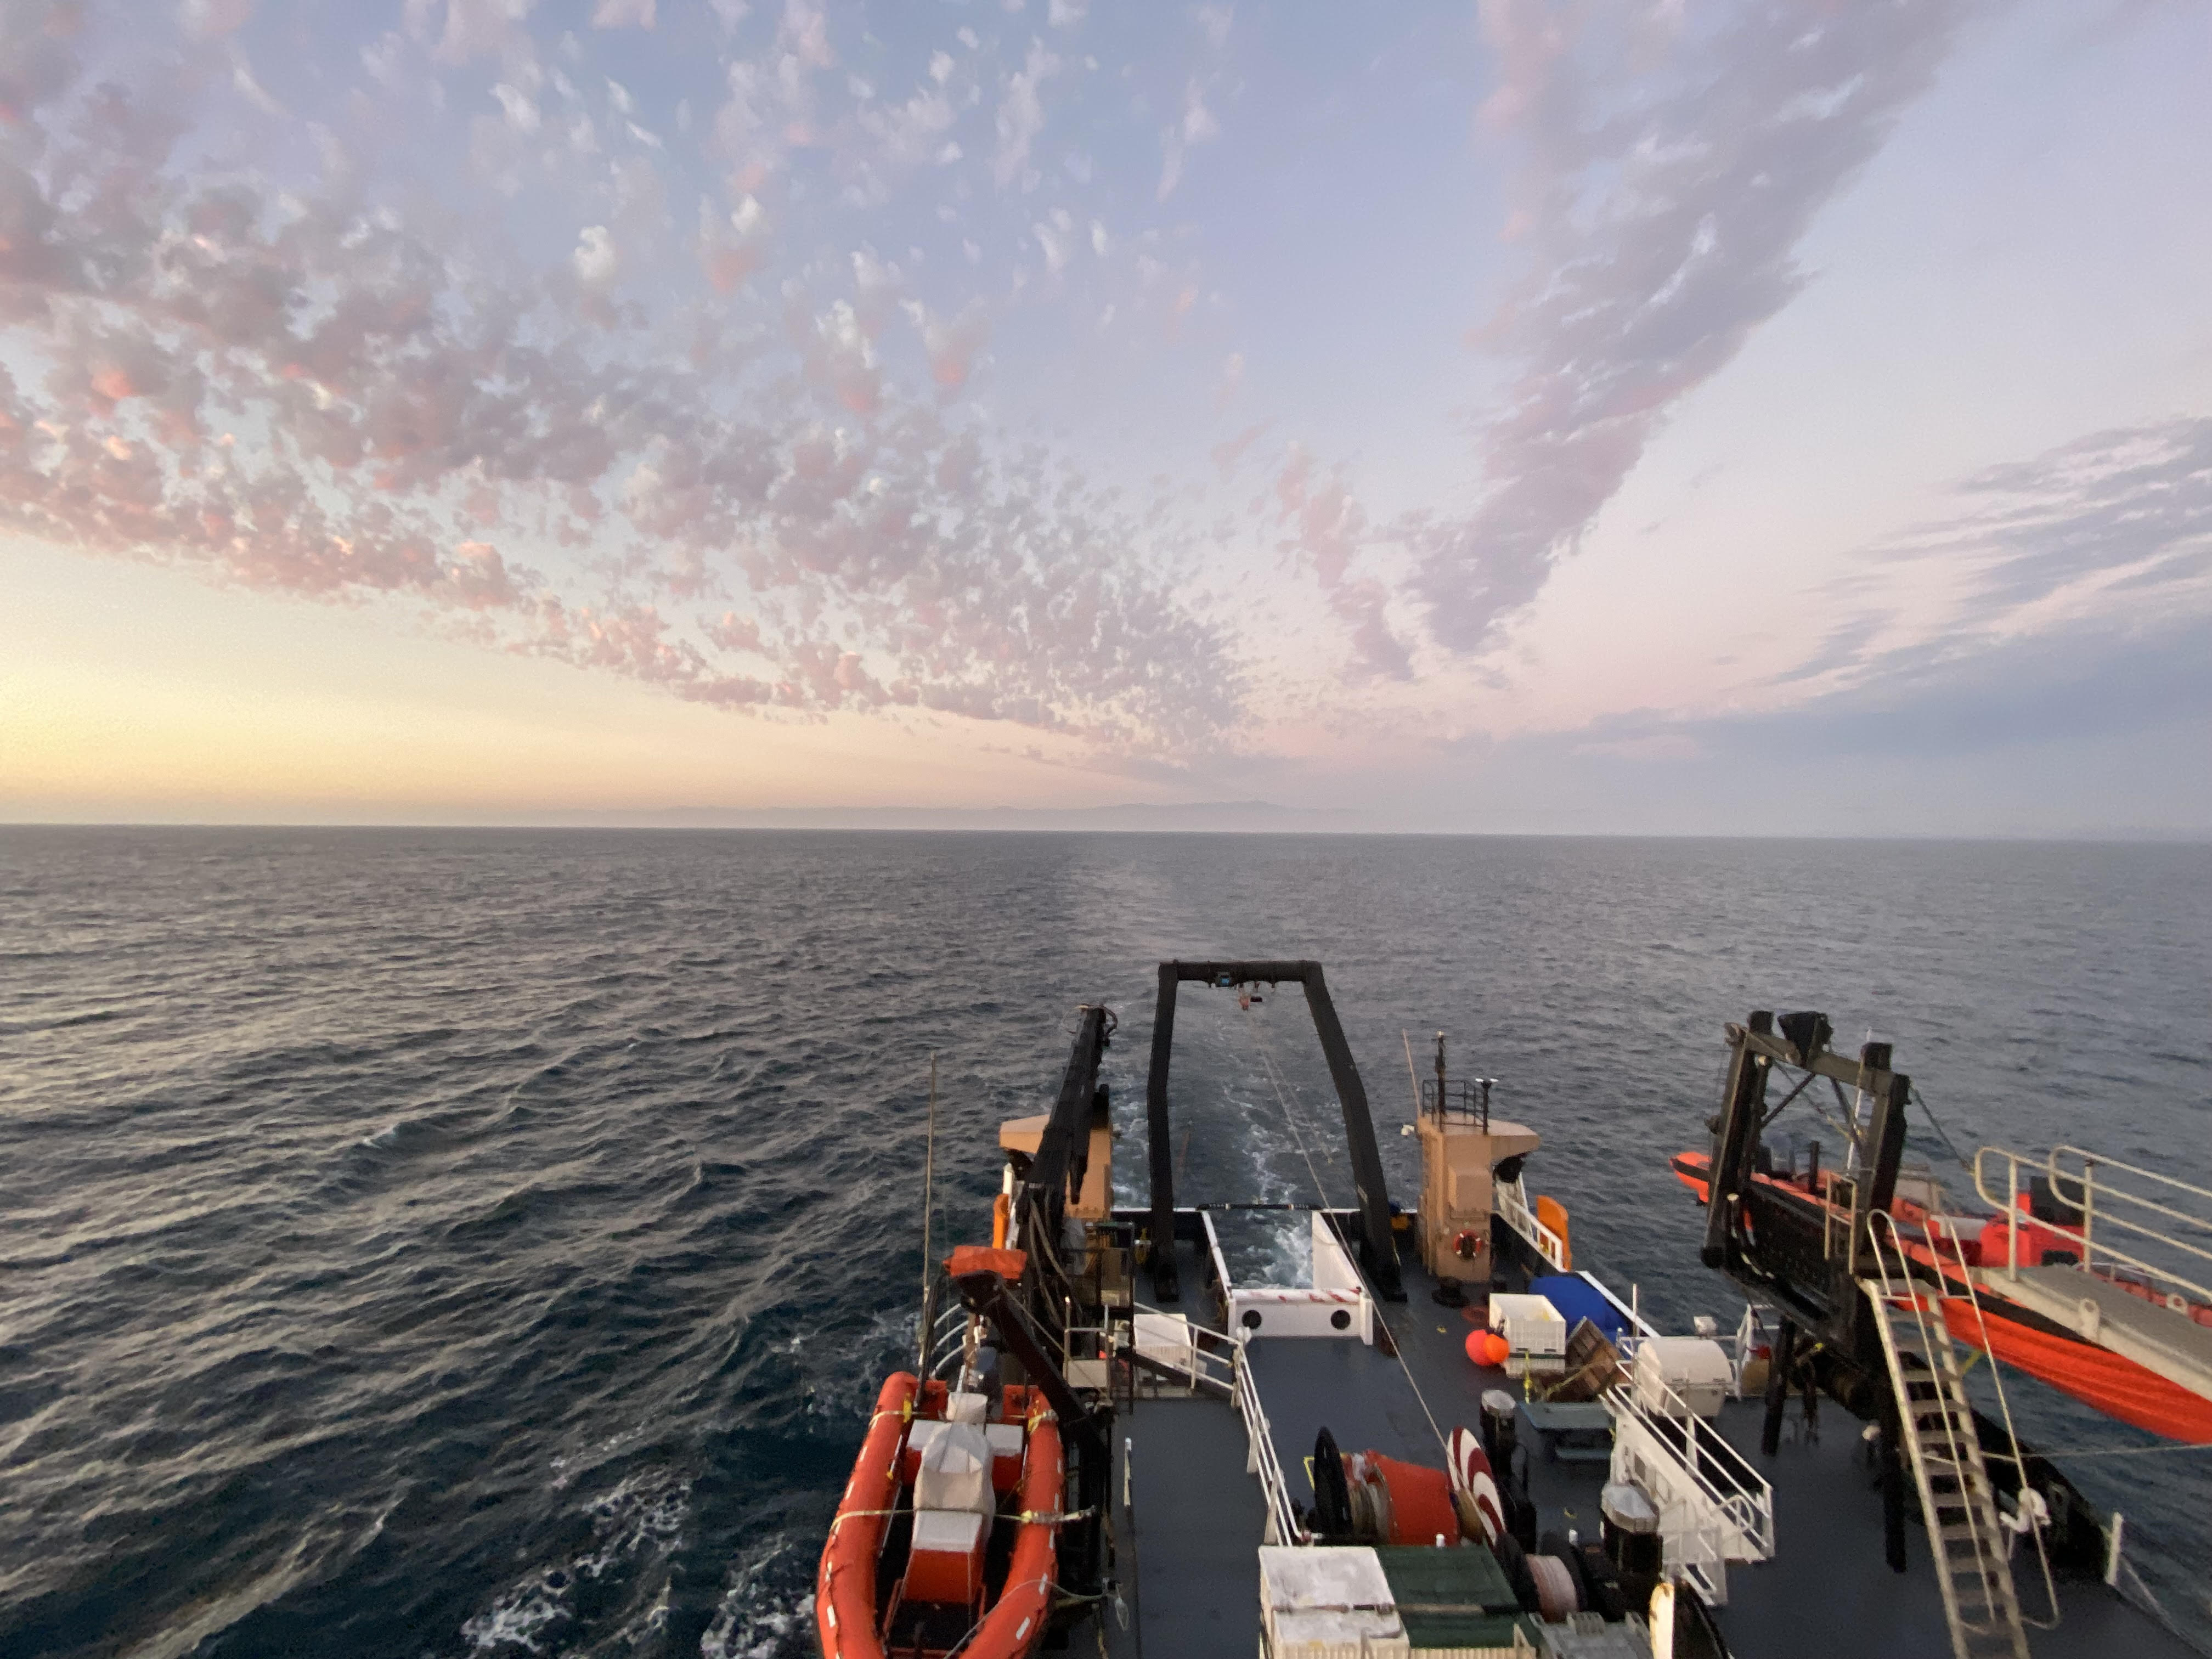
\includegraphics[width=8.20833in,height=\textheight]{content/images/lasker-sunset.jpg}

}

\caption{Survey work typically takes place on the NOAA Ship Reuben
Lasker with acoustic sampling during the day and trawl sampling at
night. Here is the back deck of the NOAA Ship Reuben Lasker at sunset .
Inside the ship the biosampling team is getting ready for a night of
trawling.}

\end{figure}%

\section*{Document Objective:}\label{document-objective}
\addcontentsline{toc}{section}{Document Objective:}

\markright{Document Objective:}

This resource demonstrate how the SWFSC uses acoustic data generate
biomass estimates of Coastal Pelagic Species. As part of our commitment
to open science, reproducibility, and transparency, we provide this
metadata guide to compliment our public-domain data. Please consider
this resource to be a~\textbf{Living Document}. The code in this
repository is regularly being updated and improved.~

Do not hesitate to reach out (to us at
either~alice.beittel@noaa.gov~or~\href{https://github.com/nmfs-swfsc-ast/echo-class/issues}{GitHub
issues}, especially if you find discrepancies in the data or want to
suggest improvements to infrastructure. Thank you in advance for your
collaboration and partnership with us as we develop our future data
universe.

\section*{User Resources}\label{user-resources}
\addcontentsline{toc}{section}{User Resources}

\markright{User Resources}

The survey produces two reports each year: A Survey Report and a Biomass
Report. Each can be found at the NOAA Institutional Repository online

\begin{itemize}
\item
  \href{https://repository.library.noaa.gov/view/noaa/61651}{2023
  Biomass Report}: \emph{Distribution, biomass, and demographics of
  coastal pelagic fishes in the California Current Ecosystem during
  summer 2023 based on acoustic-trawl sampling}
\item
  \href{https://repository.library.noaa.gov/view/noaa/61647}{2023 Survey
  Report}: \emph{Report on the Summer 2023 California Current Ecosystem
  Survey (CCES) (2307RL), 17 July to 3 November 2023, conducted aboard
  NOAA Ships Reuben Lasker and Bell M. Shimada, fishing vessels Lisa
  Marie and Long Beach Carnage, and three uncrewed surface vessels}
\end{itemize}

\section*{Cite This Data}\label{cite-this-data}
\addcontentsline{toc}{section}{Cite This Data}

\markright{Cite This Data}

{[}enter text on how to do this{]}

\section*{NOAA README}\label{noaa-readme}
\addcontentsline{toc}{section}{NOAA README}

\markright{NOAA README}

This repository is a scientific product and is not official
communication of the National Oceanic and Atmospheric Administration, or
the United States Department of Commerce. All NOAA GitHub project code
is provided on an `as is' basis and the user assumes responsibility for
its use. Any claims against the Department of Commerce or Department of
Commerce bureaus stemming from the use of this GitHub project will be
governed by all applicable Federal law. Any reference to specific
commercial products, processes, or services by service mark, trademark,
manufacturer, or otherwise, does not constitute or imply their
endorsement, recommendation or favoring by the Department of Commerce.
The Department of Commerce seal and logo, or the seal and logo of a DOC
bureau, shall not be used in any manner to imply endorsement of any
commercial product or activity by DOC or the United States Government.

\section*{NOAA License}\label{noaa-license}
\addcontentsline{toc}{section}{NOAA License}

\markright{NOAA License}

Software code created by U.S. Government employees is not subject to
copyright in the United States (17 U.S.C. §105). The United
States/Department of Commerce reserve all rights to seek and obtain
copyright protection in countries other than the United States for
Software authored in its entirety by the Department of Commerce. To this
end, the Department of Commerce hereby grants to Recipient a
royalty-free, nonexclusive license to use, copy, and create derivative
works of the Software outside of the United States.

Copyright 2024 SWFSC Advanced Survey Technology Program\\
\strut \\
Licensed under the Apache License, Version 2.0 (the ``License''); you
may not use this file except in compliance with the License. You may
obtain a copy of the License at
\url{http://www.apache.org/licenses/LICENSE-2.0}\\
\strut \\
Unless required by applicable law or agreed to in writing, software
distributed under the License is distributed on an ``AS IS'' BASIS,
WITHOUT WARRANTIES OR CONDITIONS OF ANY KIND, either express or implied.
See the License for the specific language governing permissions and
limitations under the License.

\bookmarksetup{startatroot}

\chapter{Survey Background}\label{survey-background}

\section{Who conducts the survey?}\label{who-conducts-the-survey}

The California Current Ecosystem Survey is conducted by researchers at
the NOAA Southwest Fisheries Science Center from the Fisheries Resources
Division. The survey is also made possible by volunteers from additional
NOAA line offices and science centers, universities, international
partners, NOAA interns, and inter-agency employees.

\section{Where does the survey take
place?}\label{where-does-the-survey-take-place}

\begin{figure}

\begin{minipage}{0.50\linewidth}

\begin{figure}[H]

{\centering 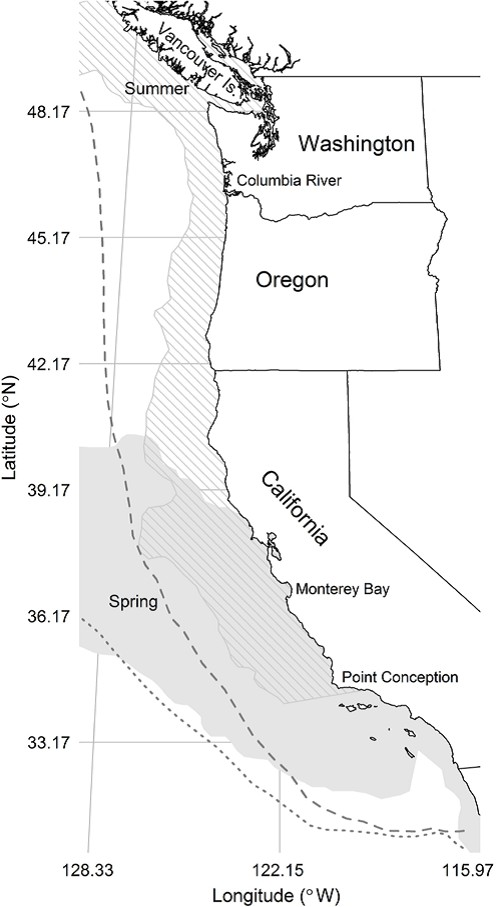
\includegraphics[width=\textwidth,height=6in]{content/images/clipboard-1472872065.png}

}

\subcaption{Sardine distribution}

\end{figure}%

\end{minipage}%
%
\begin{minipage}{0.50\linewidth}

\begin{figure}[H]

{\centering 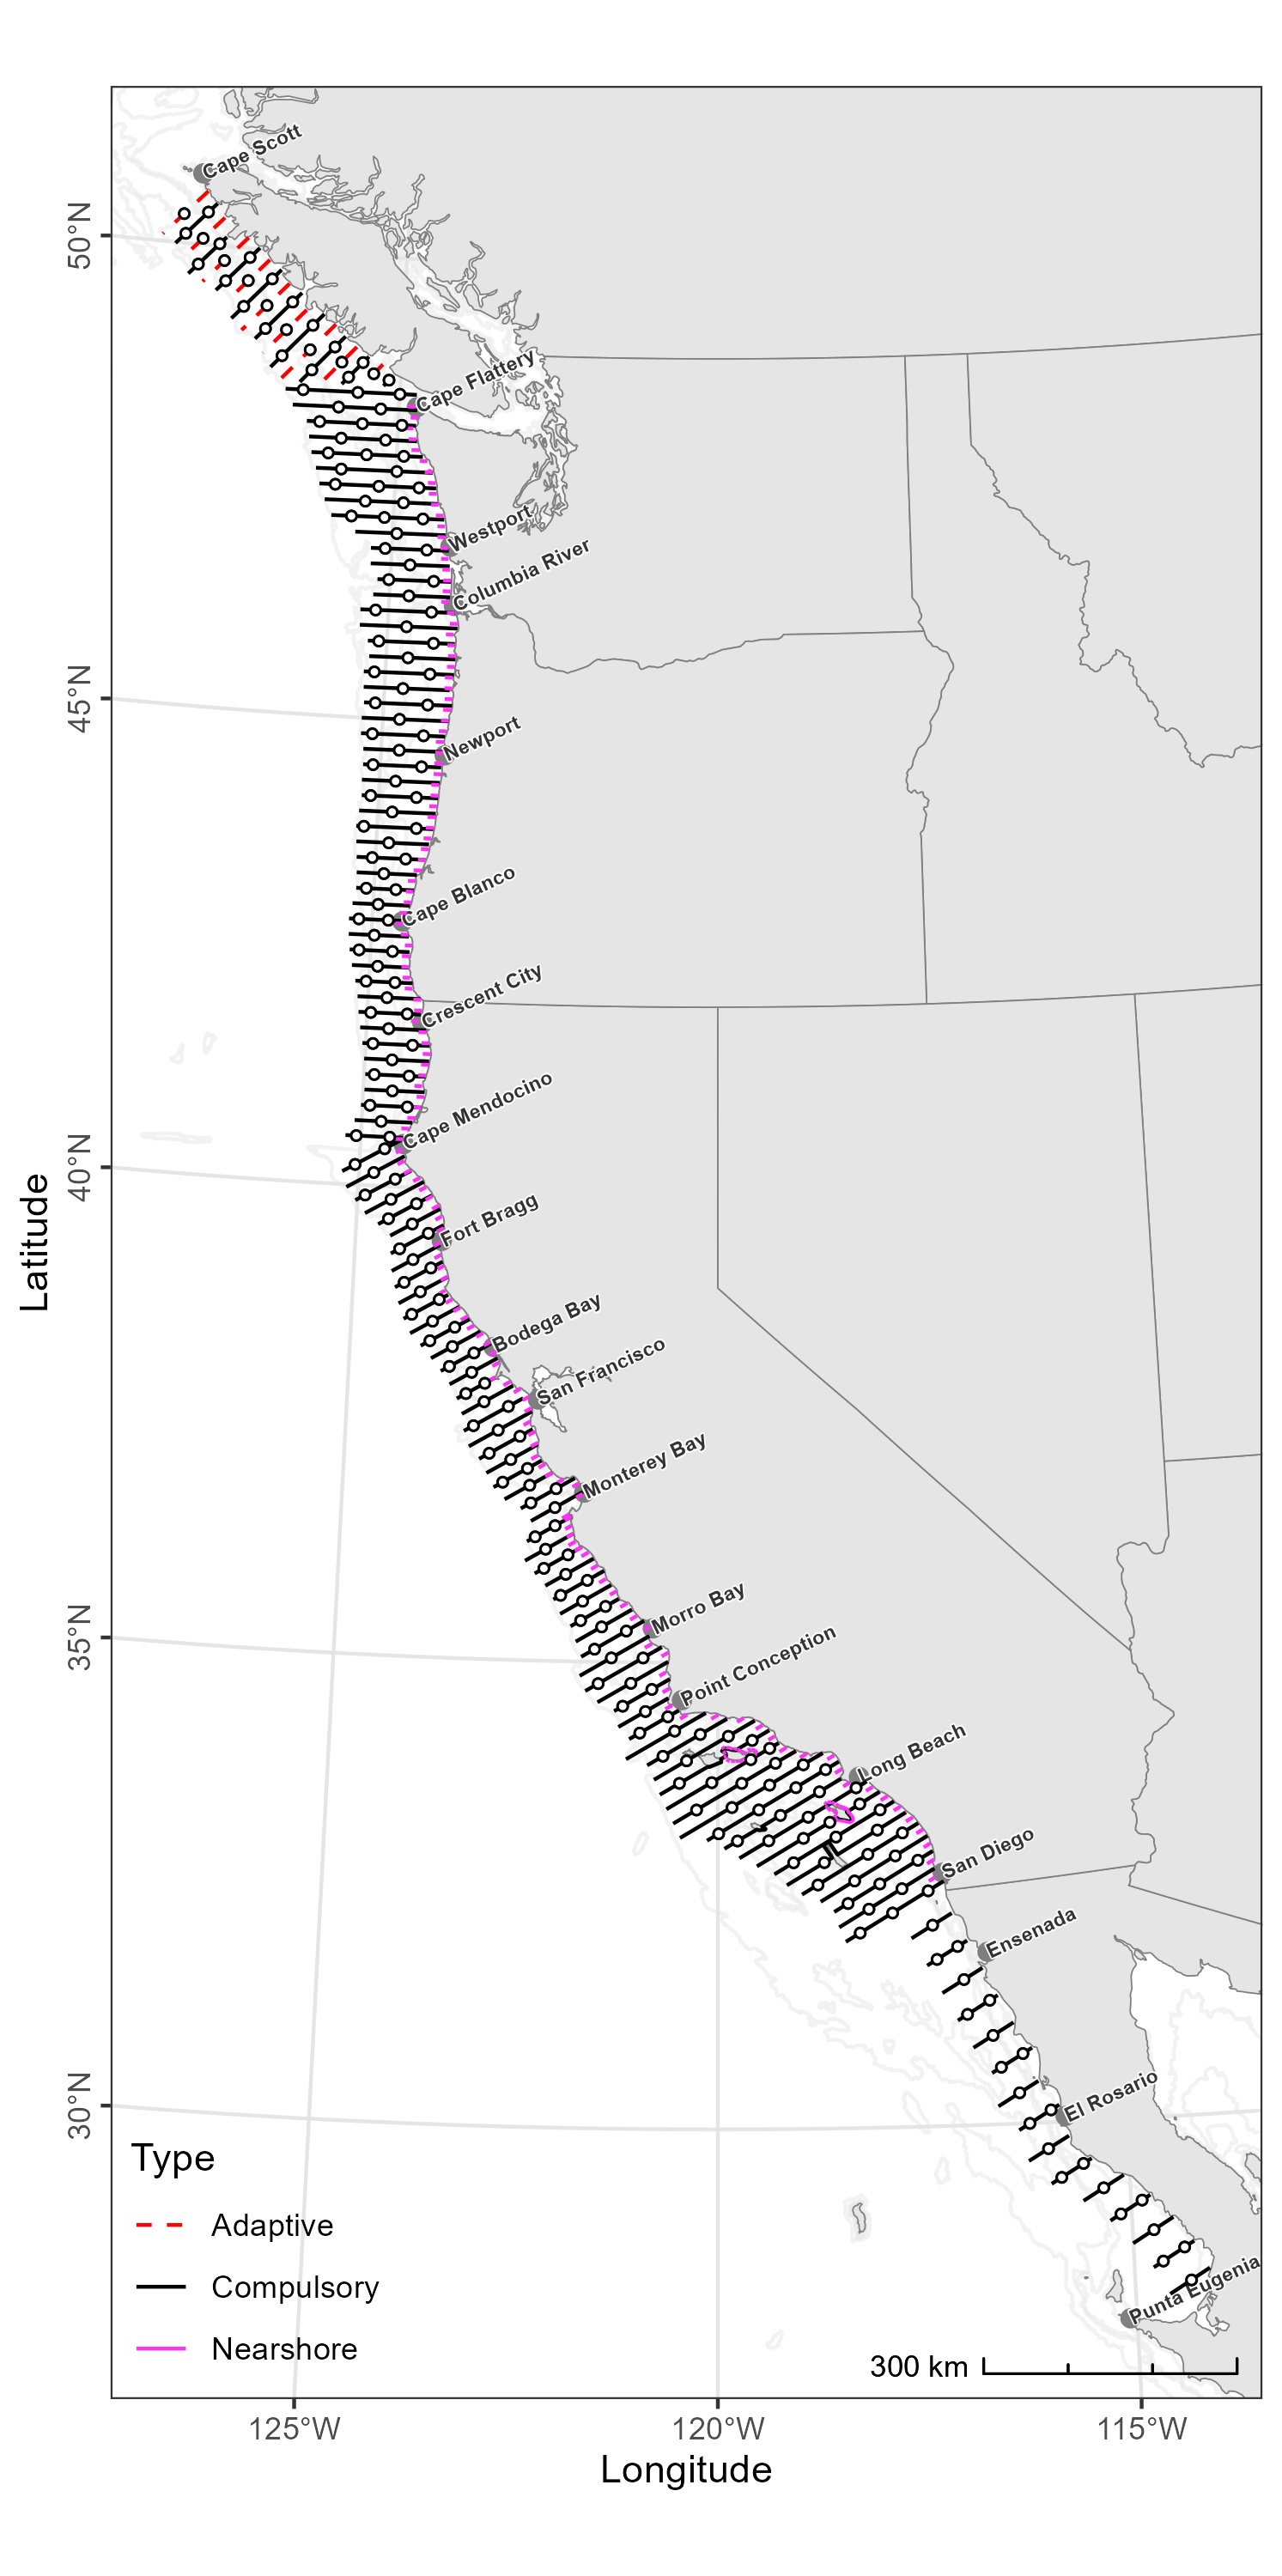
\includegraphics[width=\textwidth,height=6in]{content/images/fig_survey_map.png}

}

\subcaption{General sampling scheme}

\end{figure}%

\end{minipage}%

\caption{\label{fig-survey}On left, a conceptual spring (shaded region)
and summer (hashed region) distributions of potential habitat for the
northern stock of Pacific Sardine along the west coasts of Mexico, the
United States, and Canada. On right, the general sampling scheme of
planned core-region (solid black lines), adaptive (dashed red lines),
and nearshore lines (pink).}

\end{figure}%

\section{Research objectives:}\label{research-objectives}

\begin{enumerate}
\def\labelenumi{\arabic{enumi}.}
\tightlist
\item
  Acoustically map the distributions, measure the species compositions
  and size-frequency distributions, and estimate the abundances and
  biomasses of CPS present in the survey area, e.g., Pacific Sardine
  Sardinops sagax, Northern Anchovy (\emph{Engraulis mordax}), Pacifc
  Herring (\emph{Clupea pallasii}), Round Herring (\emph{Etrumeus
  acuminatus}), Pacific Mackerel (\emph{Scomber japonicus}), and Jack
  Mackerel (\emph{Trachurus symmetricus})
\item
  Characterize and investigate linkages to their biotic and abiotic
  environments
\item
  Gather information regarding their life histories
\item
  Compare the species composition and size distributions of trawls and
  near shore vessel purse seine sets.
\end{enumerate}

\section{Survey History:}\label{survey-history}

The SWFSC's ATM surveys of CPS in the CCE began in 2006 with a focus on
the northern stock of Pacific Sardine. Quickly the annual surveys
demonstrated valuable ecosystem insights. Since then, they have expanded
in scope and objectives to include the larger forage-fish assemblage and
krill. This evolution, and the migratory behavior of Pacific Sardine,
serve to explain the present survey region and design.

``Collectively, these annual or bi-annual ATM surveys provide a unique
insight into the dynamics of forage fshes in the CCE, including their
distributions, abundances, interactions, and environments. For example,
results from 2006 through 2013 indicate that Pacifc Sardine dominated
the CPS assemblage, but their biomass was declining (Demer and
Zwolinski, 2012; Zwolinski and Demer, 2012) and their seasonal migration
was contracting (Zwolinski et al., 2014). Meanwhile, harvest rates for
the declining stock increased (Demer and Zwolinski, 2017), and the total
forage-fsh biomass decreased to less than 200,000 t in 2014 and 2015
(Figs. 36, 37). The U.S. fshery for Pacifc Sardine was closed in 2015
(National Marine Fisheries Service, 2015), and there were reports of
mass strandings, deaths, and reproductive failures in Brown Pelicans
(Pelecanus occidentalis3), Common Murres (Uria aalge), Brandt's
Cormorants (Phalacrocorax penicillatus), and California sea lions
(Zalophus californianus4) (McClatchie et al., 2016), all of which depend
on forage species. Since 2016, the forage-fsh biomass has increased,
mainly due to resurgences of Jack Mackerel and the now dominant central
stock of Northern Anchovy (Figs. 36, 37), whose biomass primarily
(2,466,108 t, or 94\% of the total estimate biomass) occurred in U.S.
waters. Between the summers of 2018 and 2021, the biomass of the
southern stock of Pacifc Sardine in U.S. waters has increased from
33,093 to 45,332 t.''(Stierhoff et al. 2024)

\section{Code of Conduct}\label{code-of-conduct}

\subsection{What are Codes of Conduct?}\label{what-are-codes-of-conduct}

Codes of Conduct are voluntary sets of rules that assist creators,
developers, and users of code and data with data protection compliance
and accountability in specific sectors or relating to particular
processing operations.

Codes can help organizations to ensure all participants follow best
practices and rules designed specifically for their sector or processing
operations, thus enhancing compliance and collaboration. They are
developed and managed by an association or other body (the `Code Owner')
which is representative of a sector (or category of data controllers or
processors), with the expert and sectoral knowledge of how to enhance
data protection in their area.

\subsection{\texorpdfstring{\href{https://github.com/nmfs-opensci/.github/blob/main/CODE_OF_CONDUCT.md}{Code
of Conduct} from the \href{https://nmfs-opensci.github.io/}{nmfs-opensci
GitHub}.}{Code of Conduct from the nmfs-opensci GitHub.}}\label{code-of-conduct-from-the-nmfs-opensci-github.}

\bookmarksetup{startatroot}

\chapter{NOAA Fisheries Open Science Code of
Conduct}\label{noaa-fisheries-open-science-code-of-conduct}

This code of conduct was developed and adapted from the Atom code of
conduct in October 2021.

\section{Our Pledge}\label{our-pledge}

In the interest of fostering an open and welcoming environment, we as
contributors and maintainers pledge to making participation in our
project and our community a harassment-free experience for everyone,
regardless of age, body size, disability, ethnicity, gender identity and
expression, level of experience, nationality, personal appearance, race,
religion, or sexual identity and orientation.

\section{Our Standards}\label{our-standards}

Examples of behavior that contributes to creating a positive environment
include:

\begin{itemize}
\tightlist
\item
  Using welcoming and inclusive language
\item
  Being respectful of differing viewpoints and experiences
\item
  Gracefully accepting constructive criticism
\item
  Focusing on what is best for the community
\item
  Showing empathy towards other community members
\end{itemize}

Examples of unacceptable behavior by participants include:

\begin{itemize}
\tightlist
\item
  The use of sexualized language or imagery and unwelcome sexual
  attention or advances
\item
  Trolling, insulting/derogatory comments, and personal or political
  attacks
\item
  Public or private harassment
\item
  Publishing others' private information, such as a physical or
  electronic address, without explicit permission
\item
  Other conduct which could reasonably be considered inappropriate in a
  professional setting
\end{itemize}

\section{Our Responsibilities}\label{our-responsibilities}

Project maintainers are responsible for clarifying the standards of
acceptable behavior and are expected to take appropriate and fair
corrective action in response to any instances of unacceptable behavior.

Project maintainers have the right and responsibility to remove, edit,
or reject comments, commits, code, wiki edits, issues, and other
contributions that are not aligned to this Code of Conduct, or to ban
temporarily or permanently any contributor for other behaviors that they
deem inappropriate, threatening, offensive, or harmful.

\section{Scope}\label{scope}

This Code of Conduct applies both within project spaces and in public
spaces when an individual is representing the project or its community.
Examples of representing a project or community include using an
official project e-mail address, posting via an official social media
account, or acting as an appointed representative at an online or
offline event. Representation of a project may be further defined and
clarified by project maintainers.

\section{Enforcement}\label{enforcement}

Instances of abusive, harassing, or otherwise unacceptable behavior may
be reported by contacting the project team. All complaints will be
reviewed and investigated and will result in a response that is deemed
necessary and appropriate to the circumstances. Further details of
specific enforcement policies may be posted separately.

\section{Attribution}\label{attribution}

This Code of Conduct is adapted from the
\href{https://contributor-covenant.org}{Contributor Covenant}, version
1.4, available at
\href{https://contributor-covenant.org/version/1/4/}{https://contributor-covenant.org/version/1/4}

\bookmarksetup{startatroot}

\chapter{Data Acquisition}\label{data-acquisition}

\section{Survey Equipment}\label{survey-equipment}

\subsection{Acoustic Instruments}\label{acoustic-instruments}

\begin{figure}

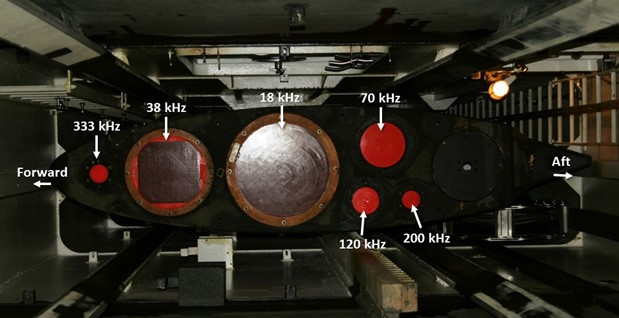
\includegraphics{content/images/transducers.jpg}

\caption{\label{fig-transducers}Transducer locations on the bottom of
the centerboard aboard Lasker.}

\end{figure}%

On \emph{Lasker} and \emph{Shimada}, multi-frequency Wideband
Transceivers (Simrad EK80 WBTs; Kongsberg) were confgured with
split-beam transducers (Simrad ES18, ES38-7, ES70-7C, ES120-7C,
ES200-7C, and ES333- 7C on \emph{Lasker} and ES18, ES38B, ES70-7C,
ES120-7C, and ES200-7C on \emph{Shimada}; Kongsberg). The transducers
were mounted on the bottom of a retractable keel or ``centerboard''
(Figure~\ref{fig-transducers}). The keel was retracted (transducers
\textasciitilde5-m depth) during calibration, and extended to the
intermediate position (transducers \textasciitilde7-m depth) during the
survey. Exceptions were made during shallow water operations, when the
keel was retracted; or during times of heavy weather, when the keel was
extended (transducers \textasciitilde9-m depth) to provide extra
stability and reduce the efect of weather-generated noise. Transducer
position and motion were measured at 5 Hz using an inertial motion unit
(Applanix POS-MV; Trimble).

\subsection{Underway CTD}\label{underway-ctd}

On \emph{Lasker} and \emph{Shimada}, conductivity and temperature
profiles were measured down to 300 m using calibrated sensors on a probe
cast from the vessel while underway (UnderwayCTD, or UCTD; Teledyne
Ocean- science). Casts were typically conducted between two to four
times along each transect. These data indicate the depth of the surface
mixed layer, above which most pelagic CPS reside during the day. These
data were also used to estimate the time-averaged sound speed (Demer,
2004), for estimating ranges to the sound scatterers, and
frequency-specific sound absorption coefficients, for compensating
signal attenuation of the sound pulse between the transducer and
scatterers (Simmonds and MacLennan, 2005).

\section{Software}\label{software}

\subsection{Echosounder Software}\label{echosounder-software}

EK80

\subsection{NetTime}\label{nettime}

On \emph{Lasker} and \emph{Shimada}, the computer clocks were
synchronized with the GPS clock (UTC) using a synchronization software
called NetTime.

\subsection{EAL}\label{eal}

The 38-, 70-, 120-, 200-, and 333-kHz echosounders were controlled by
the EK80 Adaptive Logger
(EAL\href{file:///C:/Users/alice.beittel/Downloads/2024Renfree.docx\#_bookmark7}{2},
Renfree and Demer, 2016). The EAL optimizes the pulse interval based on
the seabed depth, while avoiding aliased seabed echoes, and was
programmed such that once an hour the echosounders would record three
pings in passive mode, for obtaining estimates of the background noise
level.

\subsection{K Sync}\label{k-sync}

To minimize acoustic interference on \emph{Lasker} and \emph{Shimada},
transmit pulses from the EK80s, acoustic Doppler current profiler and
echosounder (Simrad-Kongsberg EC150-3C), multibeam echosounder (Simrad-
Kongsberg ME70), imaging sonar (Simrad-Kongsberg MS70), scanning sonar
(Simrad-Kongsberg SX90), and a separate acoustic Doppler current
profiler (Teledyne RD Instruments OS75 ADCP) were triggered using a
synchronization system (Simrad K-Sync; Kongsberg). The K-Sync trigger
rate, and thus the echosounder ping interval, was modulated by the EAL
using the 18-kHz seabed depth provided by the Scientific Computing
System (SCS).

\section{Raw Acoustic Data Format}\label{raw-acoustic-data-format}

Measurements of volume backscattering strength
(\emph{S\textsubscript{v}}; dB re 1 m2 m-3) and target strength
(\emph{TS}; dB re 1 m2), indexed by time and geographic positions
provided by GPS receivers, were stored in Simrad-Kongsberg .raw format
with a 1-GB maximum file size. During daytime, the echosounders operated
in CW mode and logged to 60 m beyond the detected seabed range or to a
maximum range of 500, 500, 500, 300, and 150 m for 38, 70, 120, 200, and
333 kHz, respectively. During nighttime, the echosounders operated in FM
mode and logged to 100 m. For each acoustic instrument, the prefix for
each fle name is a concatenation of the survey name (e.g., 2307RL), the
operational mode (CW or FM), and the logging commencement date and time
from the EK80 software (v21.15.1). For example, a file generated by the
Simrad-Kongsberg EK80 software for a WBT operated in CW mode is named
2307RL\_CW-D20220826-T155651.raw.

\bookmarksetup{startatroot}

\chapter{Data Processing}\label{data-processing}

After data aqusition, we identify acoustic echos of schooling CPS using
a semi-automated data processing algorithm using Echoview software and
in-house \texttt{Posit} code in the \texttt{estimATM}
\href{https://github.com/kstierhoff/estimATM}{repository}. With
Echoview, we extract the backscatter of swim bladder fish and process
using soundspeed and echosounder calibration values housed inside an
Echoview Calibration Supplement (\texttt{.ecs)} file. The Echoview
filters and thresholds were based on a sub-sample of echoes from
randomly selected CPS schools. We complete the processing with the
\texttt{estimATM} package in \texttt{extract\_CPS\_NASC.R}, where we
further refine the backscatter selection to extract only CPS. Here we
will cover the Echoview and \texttt{estimATM} semi-automated processing
workflow.

\subsection{Data Processing Overview}\label{data-processing-overview}

\begin{figure}[H]

{\centering 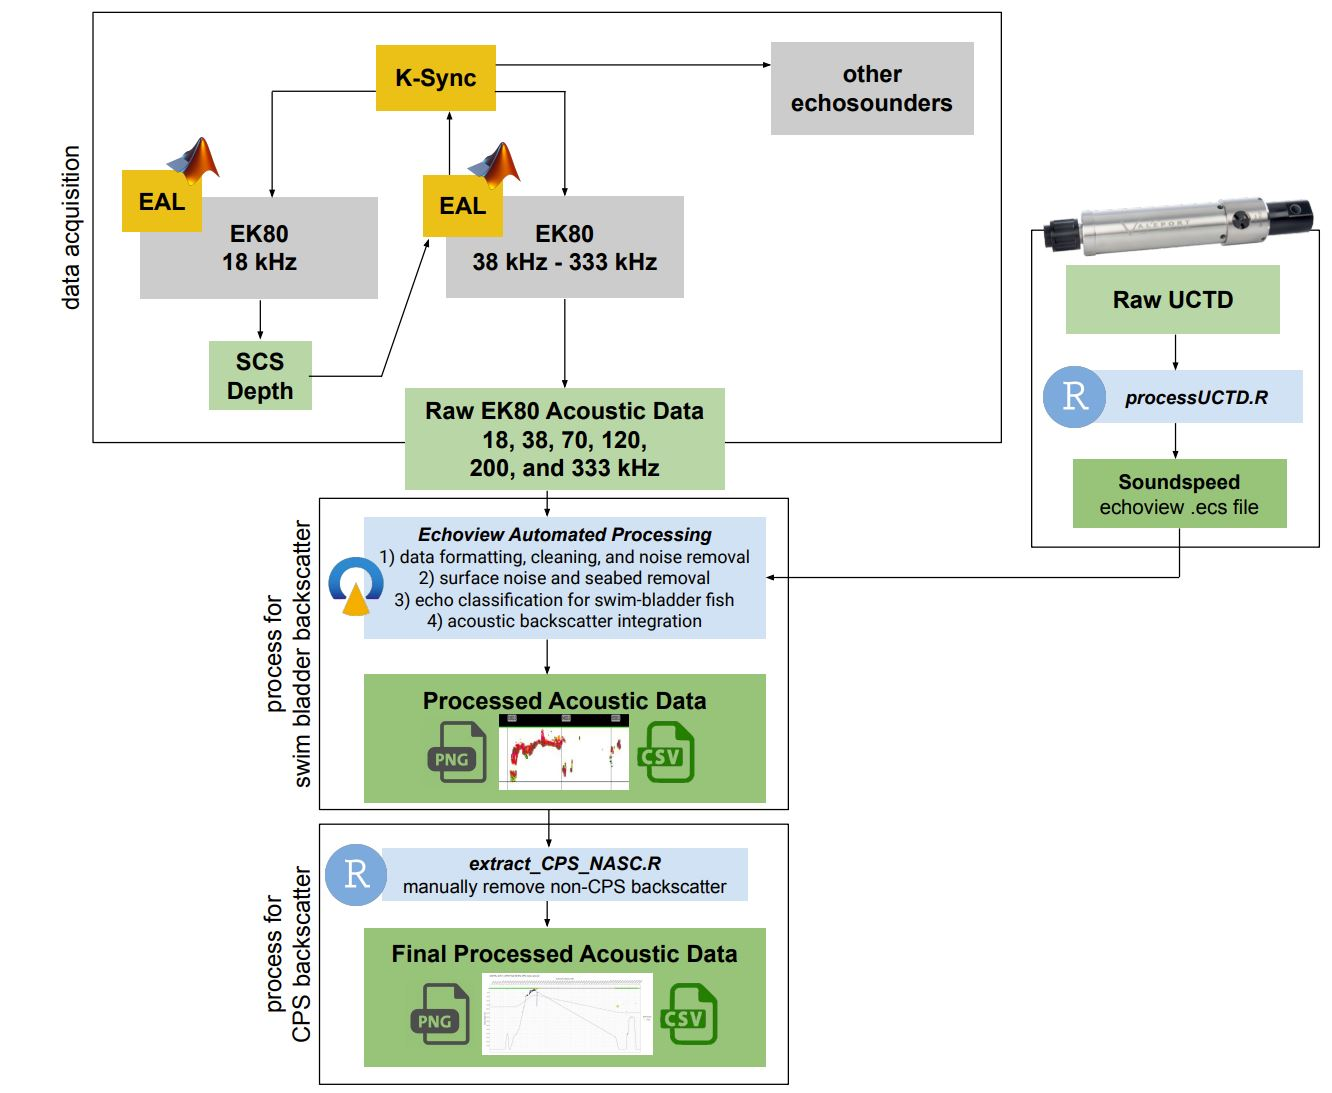
\includegraphics{content/images/processing-overview.JPG}

}

\caption{Overview of CPS Acoustic Processing. Vessel position and
attitude data is used from the POS MV (not shown).}

\end{figure}%

\begin{center}\rule{0.5\linewidth}{0.5pt}\end{center}

\subsection{Echoview Processing
Workflow}\label{echoview-processing-workflow}

In Echoview, we organize, clean, and extract acoustic backscatter of
swim bladder fish. There are three key steps to this process:

\begin{enumerate}
\def\labelenumi{\arabic{enumi}.}
\item
  Data wrangling, cleaning, and noise removal (including surface noise
  and seabed removal)
\item
  Echo classification for swim-bladdred fish
\item
  Acoustic Backscatter Integration. The aim of the filter criteria is to
  retain at least 95\% of the noise-free backscatter from CPS while
  rejecting at least 95\% of the non-CPS backscatter.
\end{enumerate}

\begin{figure}[H]

{\centering 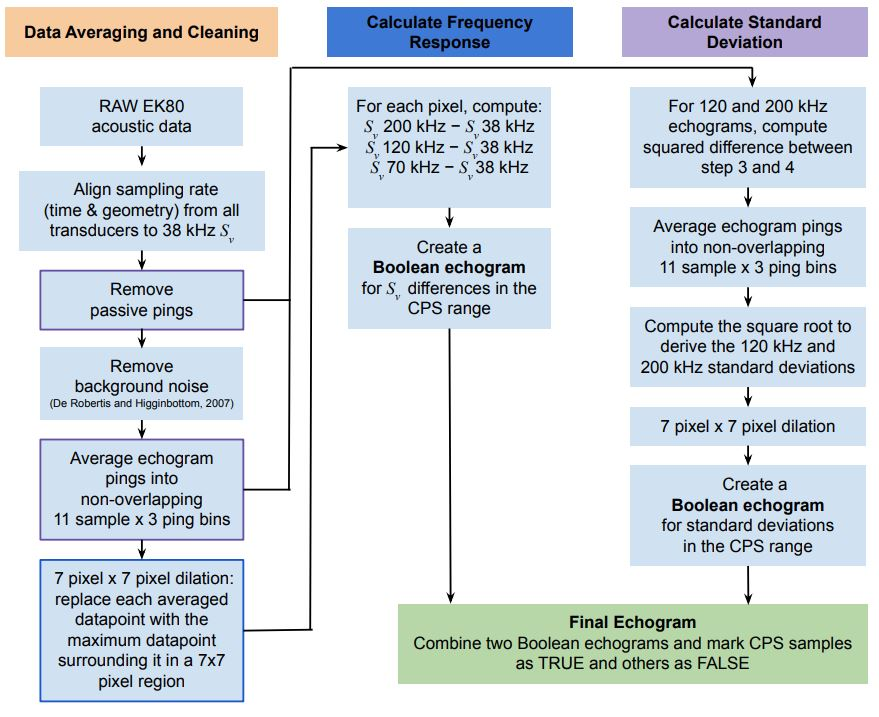
\includegraphics{content/images/ev-processing.JPG}

}

\caption{Simplified dataflow of processing in Echoview. *Surface noise
and seabed removal replies on two manual inputs: the
\texttt{Integration\ Start} and \texttt{Integration\ Stop} lines (not
pictured, see step 5).}

\end{figure}%

\subsubsection{\texorpdfstring{\textbf{Section 1) Data Wrangling,
Cleaning, and Noise
Removal:}}{Section 1) Data Wrangling, Cleaning, and Noise Removal:}}\label{section-1-data-wrangling-cleaning-and-noise-removal}

\begin{enumerate}
\def\labelenumi{\arabic{enumi}.}
\item
  Load RAW EK80 acoustic data and Echoview Calibration Supplement
  (\texttt{.ecs})file into Echoview. The \texttt{.ecs} file contains
  soundspeed information calculated from the nearest (temporally and
  spatially) Underway CTD cast and echosounder calibration parameters.
  This file is used at the very beginning to convert from power to
  \texttt{Sv} (volume-backscattering coefficient).
\item
  Align sampling rate (time and geometery) from all transders to the 38
  kHz \texttt{Sv}. Acousticians call this step `matching geometry' of
  all \texttt{Sv} variables. Making sure pings are aligned from all
  echosounders is important for calculating the frequency response of
  backscatter in steps later on.
\item
  Remove passive-mode pings.
\item
  Noise removal: estimate and subtract background noise using the
  background noise removal function described in De Robertis and
  Higginbottom (2007).
\item
  \textbf{Surface noise and seabed removal} is completed by manually
  drawing an \texttt{Integration\ Start} and \texttt{Integration\ Stop}
  line in Echoview. The \texttt{Integration\ Start} line is drawn at the
  shallowest depth to include surface CPS schools but exclude transducer
  ring down and surface noise due to sea state (typically around 5
  meters below the transducer face or \textasciitilde10m depth). The
  \texttt{Integration\ Stop} line is drawn closest to the seabed to
  include bottom dwelling animals but exclude any non-living seabed
  features (typically 3 m above the estimated seabed (Demer et al. 2009)
  or to the maximum logging range (e.g., 350 m), whichever is
  shallowest). When drawing the lines, we set the color scale to a
  minimum Sv threshold of -60 dB which corresponds to a density of
  approximately three 20-cm-long Pacific Sardine per 100 m3). Doing this
  helps visually pick out schools from the seabed and from non-swim
  bladder animals that appear as diffuse scattering layers in the water
  column. The area of the water column between the two lines sets the
  depth range that will be integrated for swim bladder fish in steps
  later on.
\item
  Average the noise-free Sv echograms using non-overlapping 11-sample by
  3-ping bins.
\item
  Expand the averaged, noise-reduced Sv echograms with a 7 pixel x 7
  pixel dilation. This replaces each averaged datapoint from Step 6 with
  the maximum datapoint surrounding it in a 7x7 pixel region.
\end{enumerate}

\subsubsection{\texorpdfstring{\textbf{Section 2) Echo Classification
for Swim Bladder
Fish}}{Section 2) Echo Classification for Swim Bladder Fish}}\label{section-2-echo-classification-for-swim-bladder-fish}

\paragraph{\texorpdfstring{\emph{Calculate Frequency
Response}:}{Calculate Frequency Response:}}\label{calculate-frequency-response}

\begin{enumerate}
\def\labelenumi{\arabic{enumi}.}
\item
  For each dilated pixel, compute:

  \texttt{Sv} 200kHz − \texttt{Sv} 38kHz

  \texttt{Sv} 120kHz − \texttt{Sv} 38kHz

  \texttt{Sv} 70kHz − \texttt{Sv} 38kHz

  The difference between \texttt{Sv} values provides the frequency
  response for those pixels. Swim bladder fish have a unique frequency
  response which we can use extract those acoustic returns in the next
  step. Acoustic returns that fall within the \texttt{Sv} ranges below
  are flagged as meeting the criteria for typical swim bladder fish,
  including CPS.
\item
  Create a Boolean echogram for \texttt{Sv} differences in the CPS
  range:

  −13.85 \textless{} \texttt{Sv} 70kHz − \texttt{Sv} 38kHz \textless{}
  9.89

  − 13.5 \textless{} \texttt{Sv} 120kHz −\texttt{Sv} 38kHz \textless{}
  9.37

  − 13.51 \textless{} \texttt{Sv} 200kHz − \texttt{Sv} 38kHz \textless{}
  12.53
\end{enumerate}

\paragraph{\texorpdfstring{\emph{Calculate Standard
Deviation}:}{Calculate Standard Deviation:}}\label{calculate-standard-deviation}

\begin{enumerate}
\def\labelenumi{\arabic{enumi}.}
\item
  For 120 and 200 kHz, compute the squared difference between the
  noise-filtered Sv (remove passive pings) and averaged Sv (11-sample x
  3 ping bin averages).
\item
  Average the results using an 11-sample by 3-ping window to derive
  variance.
\item
  Compute the square root to derive the 120- and 200-kHz standard
  deviations (σ120kHz and σ200kHz, respectively).
\item
  Expand the standard deviation echograms with a 7 pixel x 7 pixel
  dilation (same step as Section 1, Step 7).
\item
  Create a Boolean echogram based on the standard deviations in the CPS
  range:

  σ120kHz \textgreater{} -65 dB

  σ200kHz \textgreater{} -65 dB

  Diffuse backscattering layers have low σ (J. P. Zwolinski et al. 2010)
  whereas fish schools have high σ. Intersect the two Boolean echograms
  to create an echogram with ``TRUE'' samples for candidate CPS schools
  and ``FALSE'' elsewhere. Mask the noise-reduced echograms using the
  CPS Boolean echogram .
\end{enumerate}

\subsubsection{\texorpdfstring{\textbf{Section 3) Acoustic Backscatter
Integration}}{Section 3) Acoustic Backscatter Integration}}\label{section-3-acoustic-backscatter-integration}

\begin{enumerate}
\def\labelenumi{\arabic{enumi}.}
\tightlist
\item
  Integrate the volume backscattering coefficients (sV , m2 m-3)
  attributed to CPS over 5-m depths and averaged over 100-m distances;
\item
  Output the resulting nautical area scattering coefficients (sA; m2
  nmi-2) and associated information from each transect and frequency to
  comma-delimited text (.csv) files.
\end{enumerate}

\begin{center}\rule{0.5\linewidth}{0.5pt}\end{center}

\subsection{\texorpdfstring{\texttt{Posit} Processing
Workflow}{Posit Processing Workflow}}\label{posit-processing-workflow}

The exported \texttt{.csv} file from Echoview contains all swim bladder
backscatter which can include non-target species such as rockfish. In
order to further refine the acoustic classification to retain only CPS
backscatter, the processed \texttt{.csv} file proceeds to the final
semi-automated processing step in \texttt{Posit} using
\texttt{extract\_CPS\_NASC.R}, an R-based tool in the \texttt{estimATM}
package.

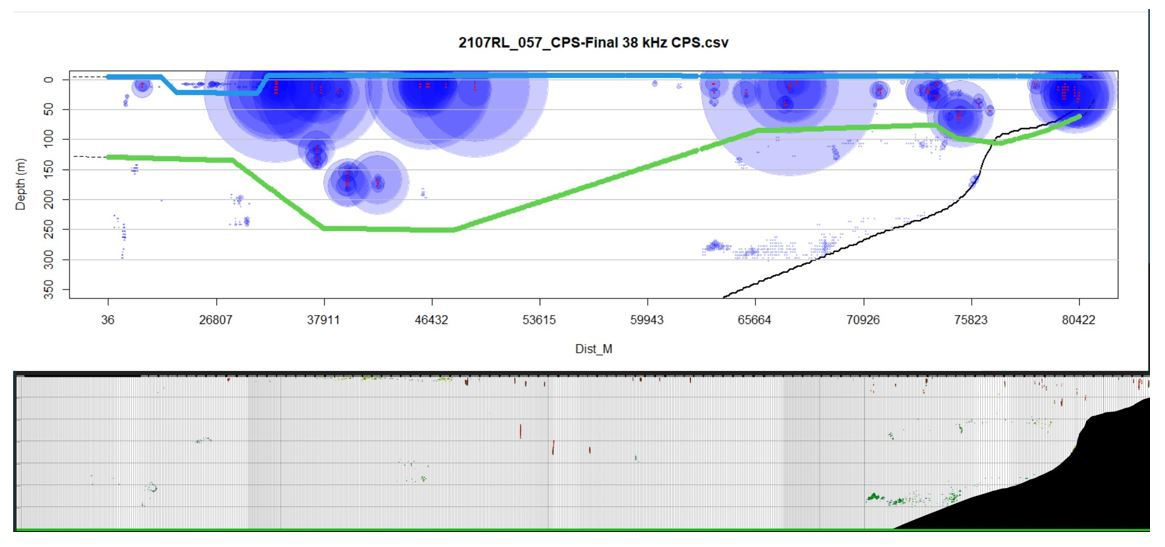
\includegraphics{content/images/nascr_processing.JPG}

Echoes from fishes with swimbladders (blue points, scaled by backscatter
intensity) along an example acoustic transect (top) and the
corresponding Echoview echogram image (bottom). In this example, the
upper (blue) and lower lines (green) indicate boundaries within which
echoes were retained. When the lower boundary is deeper than the seabed
(black line), echoes above the seabed are retained. Echoes from deep,
bottom-dwelling schools of non-CPS fishes with swimbladders, and from
diffuse scatters near the surface are excluded.

The script will open a plot (top) where the acoustics technician can
draw new integration start line (blue) and stop line (green). Blue
points that fall below the stop line will be excluded while blue points
below the start line will be included from the resulting \texttt{.csv}
file. The goal is to visually review the Echoview exported echogram
image (bottom) and remove backscatter that you believe are not CPS
(e.g., rockfishes, hake), possibly contain accidental seabed, or any
surface noise amd diffuse scattering layers. The process of picking out
CPS from other swim-bladder fish can be tricky as CPS can have a range
of characteristics. The
\href{https://nmfs-swfsc-ast.github.io/echo-class/content/identification.html}{Backscatter
Identification} section goes into detail on this process.

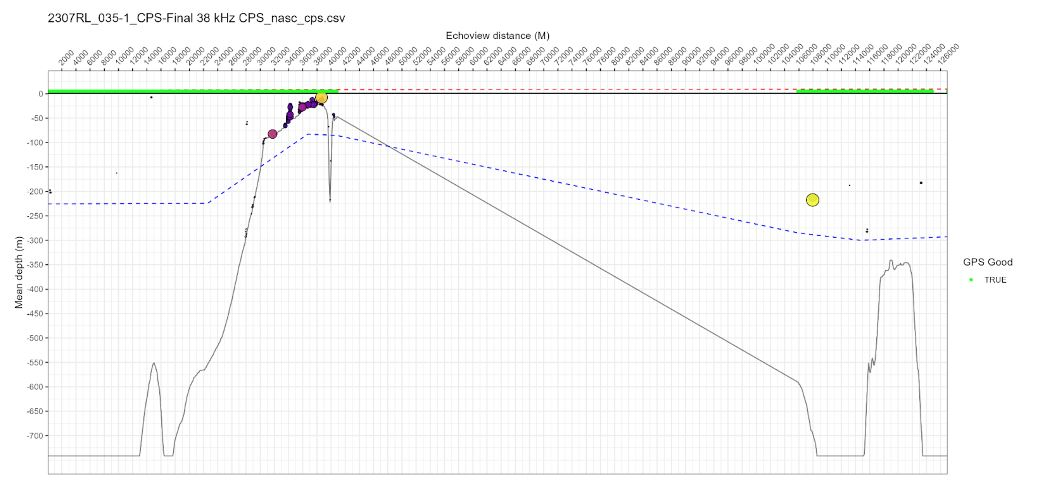
\includegraphics{content/images/nascr_processing_result.JPG}

Once you are happy with the two lines, an image will appear showing the
results of your editing. If the backscatter needs to be removed, or put
back, you can re-run the script and the results will be replaced.

\textbf{The result is a final \texttt{.csv} with only backscatter
information for CPS targets.}

\bookmarksetup{startatroot}

\chapter{Backscatter Identification}\label{backscatter-identification}

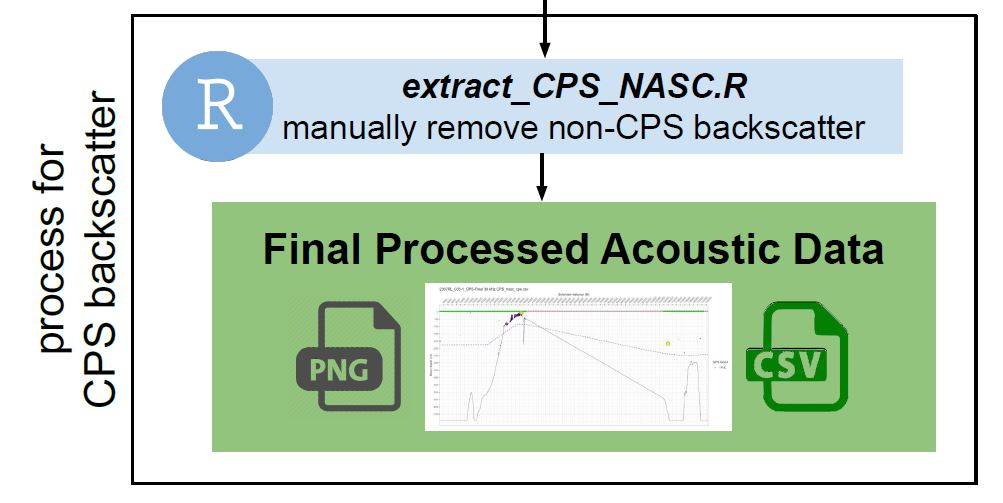
\includegraphics[width=7.29167in,height=\textheight]{content/images/processing-CPS.JPG}

When performing the final step in CPS backscatter processing, there are
several assumptions and acoustic characteristics about CPS that allow us
to refine our classification. This process aims to distinguish CPS from
non-target species from mid-water, demersal, and benthic swim bladder
fishes.

\subsubsection{Acoustic Characteristics of
CPS}\label{acoustic-characteristics-of-cps}

While the acoustic properties of swimbladder fish depends on several
factors, the most important are the acoustic wavelength, swimbladder
size, and swimbladder orientation to the incident sound pulse. We use
39, 70, 120, and 200kHz to capture a range of swimbladder sizes and
orientations. We estimate the dorsal surface area of a swimbladder
(swimbladder size) based on a function of fish lengths sampled from
nightly trawl catches. Knowing the approximate dorsal surface area of a
swimbladder allows us to calcualte an acoustic backscattering
coefficeint and derive a target strength for each CPS species. For this
survey we calculate target strength as a logarithmic function of
frequency and species-specific parameters obtained theoretically or
experimentally and fish total length from trawl samples. Full details on
species-specific target strength parameters can be found in the survey
biomass report
\href{chrome-extension://efaidnbmnnnibpcajpcglclefindmkaj/https://swfsc-publications.fisheries.noaa.gov/publications/CR/2024/2024Stierhoff.pdf}{here}.

When looking at Echoview echograms of acoustic transects, visually we
look for how the volume backscattering strength (\texttt{Sv)} changes
over each frequency. We refer to this as the frequency response.
Swimbladder fish are expected to have a flat or decreasing frequency
response across 38kHz, 70kHz, 120kHz, and 200kHz (cite image).

\phantomsection\label{frequency}
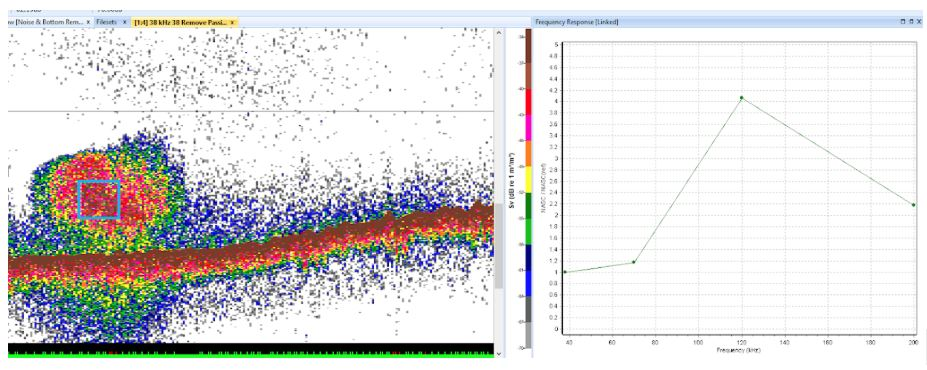
\includegraphics{content/images/CPS-freq-response.JPG}

\subsubsection{\texorpdfstring{\textbf{Biological Characteristics of
CPS}}{Biological Characteristics of CPS}}\label{biological-characteristics-of-cps}

\begin{itemize}
\item
  Temperature ranges from 8 deg C to 24 deg C and salinity from 30-38
  psu (J. P. Zwolinski et al. 2010)
\item
  Diffuse schools observed offshore near the surface or deeper than
  \textasciitilde250m
\item
  Rockfish tend to be located in areas where the seabed is hard and
  rugged
\end{itemize}

A picture guide for helping decipher tricky backscatter in the R script
extract\_CPS\_NASC.R and Echoview processing.

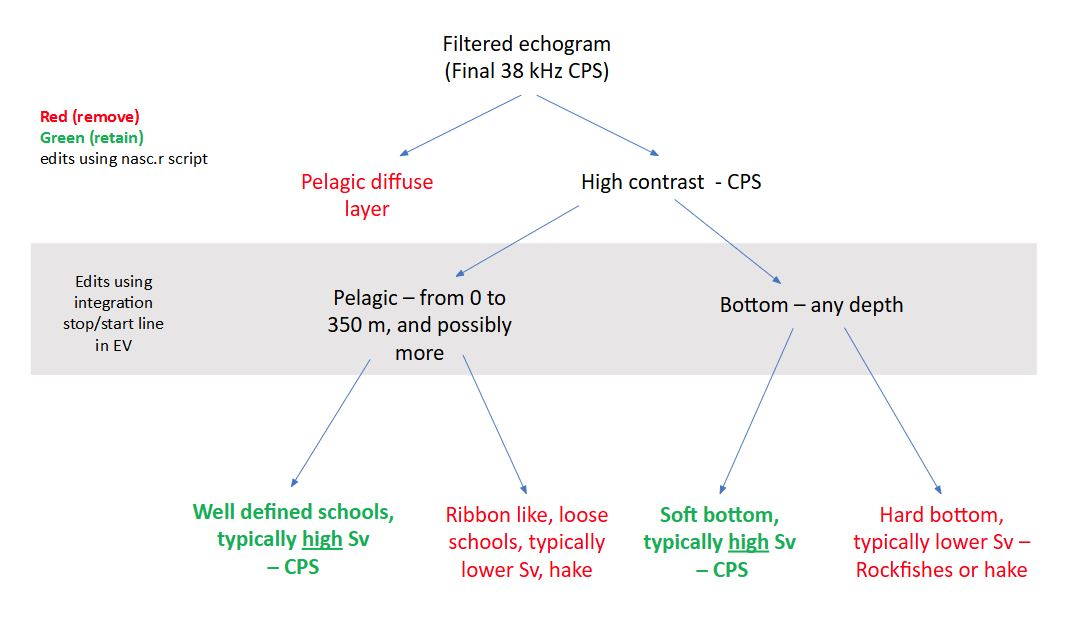
\includegraphics{content/images/backscatter_decision_tree.JPG}

Build out from
\href{https://docs.google.com/document/d/1-YxJs1veotnSZJIWPH6vJjYOA5Dt1iETaqmNv8eNoTk/edit?tab=t.0}{this
google document}.

\bookmarksetup{startatroot}

\chapter{Trawl Selection}\label{trawl-selection}

Acoustic transects are processed for CPS backscatter on the day of
acquisition and used to determine nightly trawl locations. This page
will walk through the process of trawl selection.

\subsection{\texorpdfstring{\textbf{1. Visual
Comparison}}{1. Visual Comparison}}\label{visual-comparison}

The acoustics technician on watch completes a visual comparison between
an in-house published map (plotSurvey) of backscatter results and the
transect acoustic echogram. Dense schools of CPS seen in the echogram
will correlate to colorful bubbles on plotSurvey.

\begin{enumerate}
\def\labelenumi{\arabic{enumi}.}
\item
  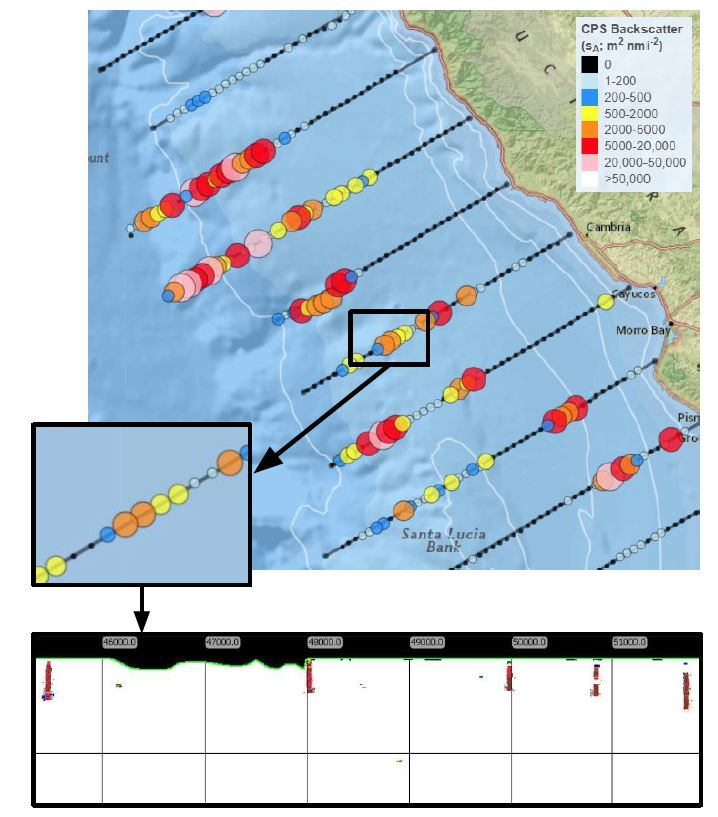
\includegraphics[width=5.63542in,height=\textheight]{content/images/trawl-selection-plotsurvey-056C.JPG}

  Clicking on summarized acoustic points shows a popup that contains the
  time and distance interval over which those data were summarized,
  allowing you to scrutinize the results of Echoview processing. We make
  sure to cross-reference backscatter spots on plotSurvey with the
  exported image from Echoview to make an informed trawl-location
  decision.

  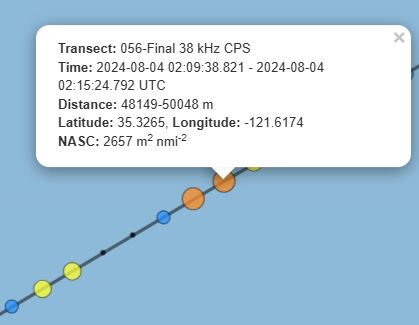
\includegraphics[width=3.51042in,height=\textheight]{content/images/trawl-selection-plotsurvey-backscatter.JPG}
\item
  The acoustics technician will select 2-3 trawls each night based on
  the backscatter observed during the daytime acoustic transect,
  operational efficiency, and expected CPS habitat. If no CPS
  backscatter is observed, trawl locations will default to using
  expected CPS habitat information and operational efficiency.
\end{enumerate}

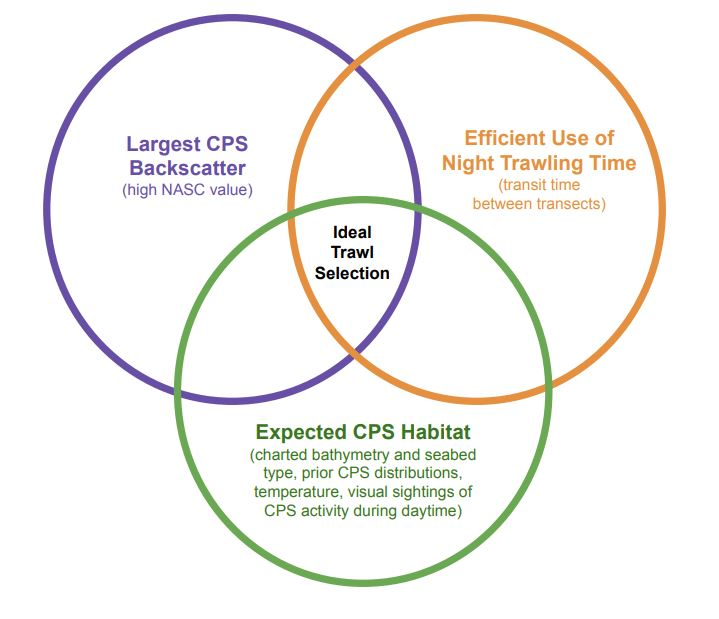
\includegraphics[width=6.6875in,height=\textheight]{content/images/trawl-selection.JPG}

Expected CPS habitat is derived from prior survey results and models:

\begin{itemize}
\item
  Sardine habitat based on a 12-year data set of sardine eggs, remotely
  sensed oceanographic variables, sea surface temperature, chlorophyll
  \emph{a} concentrations, sea surface altitude (J. P. Zwolinski,
  Emmett, and Demer 2011).
\item
  Charted bathymetry -- Pacific sardines can be found from the ocean
  surface to \textasciitilde350m in depth and typically reside around
  smoother (less rocky) bottom types.
\item
  Sardine eggs are most abundant at sea-surface temperatures of 13 to 15
  ∘C, and larvae are most abundant at 13 to 16 ∘C. Temperature is a
  primary driver of the spatial and seasonal distribution of spawning.
  During warm ocean conditions, sardine spawning shifts northward
  concentrating in offshore regions and north of Point Conception to San
  Francisco and in some years is observed as far north as Oregon
  (Kuriyama, Zwolinski, and Hill 2020).
\end{itemize}

\bookmarksetup{startatroot}

\chapter{Biomass Calculation}\label{biomass-calculation}

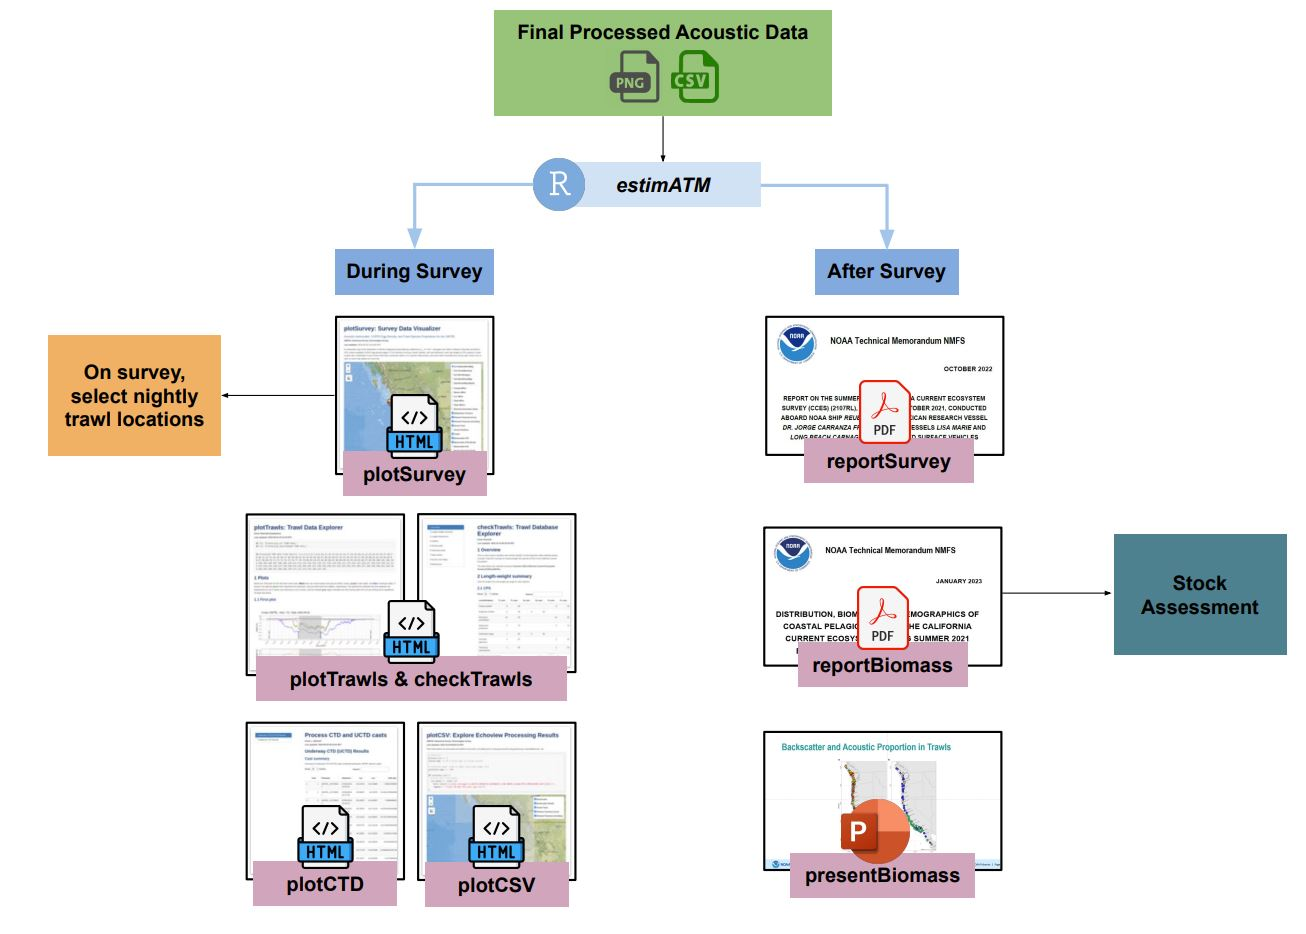
\includegraphics{content/images/estimATM_dataflow.JPG}

\bookmarksetup{startatroot}

\chapter*{References}\label{references}
\addcontentsline{toc}{chapter}{References}

\markboth{References}{References}

\phantomsection\label{refs}
\begin{CSLReferences}{1}{0}
\bibitem[\citeproctext]{ref-derobertis2007}
De Robertis, Alex, and Ian Higginbottom. 2007. {``A Post-Processing
Technique to Estimate the Signal-to-Noise Ratio and Remove Echosounder
Background Noise.''} \emph{ICES Journal of Marine Science} 64 (6):
1282--91. \url{https://doi.org/10.1093/icesjms/fsm112}.

\bibitem[\citeproctext]{ref-demer2009}
Demer, David A., George R. Cutter, Josiah S. Renfree, and John L.
Butler. 2009. {``A Statistical-Spectral Method for Echo
Classification.''} \emph{ICES Journal of Marine Science} 66 (6):
1081--90. \url{https://doi.org/10.1093/icesjms/fsp054}.

\bibitem[\citeproctext]{ref-kuriyama2020}
Kuriyama, Peter T., Juan P. Zwolinski, and Kevin T. Hill. 2020.
{``Assessment of the Pacific Sardine Resource in 2020 for u.s.
Management in 2020-2021.''} \emph{Southwest Fisheries Science Center
(U.S.)}. \url{https://doi.org/10.25923/R2FZ-4Y79}.

\bibitem[\citeproctext]{ref-stierhoff2024}
Stierhoff, Kevin L., Juan P. Zwolinski, Josiah S. Renfree, and David A.
Demer. 2024. {``Distribution, Biomass, and Demographics of Coastal
Pelagic Fishes in the California Current Ecosystem During Summer 2023
Based on Acoustic Trawl Sampling.''} \emph{NOAA National Marine
Fisheries Service Southwest Fisheries Science Center}.
\url{https://doi.org/10.25923/1VGS-SF98}.

\bibitem[\citeproctext]{ref-zwolinski2011}
Zwolinski, Juan P., Robert L. Emmett, and David A. Demer. 2011.
{``Predicting Habitat to Optimize Sampling of Pacific Sardine (Sardinops
Sagax).''} \emph{ICES Journal of Marine Science} 68 (5): 867--79.
\url{https://doi.org/10.1093/icesjms/fsr038}.

\bibitem[\citeproctext]{ref-zwolinski2010}
Zwolinski, Juan P., Paulo B. Oliveira, Victor Quintino, and Yorgos
Stratoudakis. 2010. {``Sardine Potential Habitat and Environmental
Forcing Off Western Portugal.''} \emph{ICES Journal of Marine Science}
67 (8): 1553--64. \url{https://doi.org/10.1093/icesjms/fsq068}.

\bibitem[\citeproctext]{ref-Zwolinski2014}
Zwolinski, Juan, David Demer, George Cutter, Kevin Stierhoff, and
Beverly Macewicz. 2014. {``Building on Fisheries Acoustics for Marine
Ecosystem Surveys.''} \emph{Oceanography} 27 (4): 68--79.
\url{https://doi.org/10.5670/oceanog.2014.87}.

\end{CSLReferences}


\backmatter

\end{document}
